We can use the original Zielonka's recursive algorithm to solve VPGs, to do so we will first consider a method of creating a parity game from a VPG, called \textit{unification}.
\subsection{Unified parity games}
We can create a PG from a VPG by taking all the projections of the VPG, which are PGs, and combining them into one PG by taking the union of them. We call the resulting PG the \textit{unification} of the VPG. A parity game that is the result of a unification is called a \textit{unified PG}, also any total subgame of it will be called a unified PG. A unified PG always has a VPG from which it originated.
\begin{definition}
	Given VPG $\hat{G} = (\hat{V},\hat{V}_0,\hat{V}_1, \hat{E},\hat{\Omega}, \mathfrak{C},\theta)$ we define the unification of $\hat{G}$, denoted as $\hat{G}_{\downarrow}$, as
	\[  \hat{G}_{\downarrow} = \biguplus_{c\in \mathfrak{C}}\hat{G}_{|c} \]
	where the union of two PGs is defined as
	\[ (V,V_0,V_1,E,\Omega) \uplus (V',V_0',V_1',E',\Omega') = (V \uplus V', V_0 \uplus V_0', V_1 \uplus V_1', E \uplus E', \Omega \uplus \Omega') \]
\end{definition}
We will use the hat decoration ($\hat{G},\hat{V},\hat{E},\hat{\Omega},\hat{W}$) when referring to a VPG and use no hat decoration when referring to a PG.

Every vertex in game $\hat{G}_{\downarrow}$ originates from a configuration and an original vertex. Therefore we can consider every vertex in a unification as a pair consisting of a vertex and a configuration, ie. $V = \mathfrak{C} \times \hat{V}$. We can consider edges in a unification similarly, so $E \subseteq (\mathfrak{C} \times \hat{V}) \times (\mathfrak{C} \times \hat{V})$. Note that edges don't cross configurations so for every $((c,\hat{v}) , (c',\hat{v}')) \in E$ we have $c = c'$. Figure \ref{fig:VPG2UPG} shows an example of a unification.

\begin{figure}[h]
	\centering
	\begin{subfigure}{1\textwidth}
		\centering
		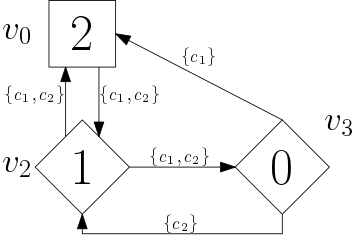
\includegraphics[scale=0.4]{Examples/UPG/VPG}
		\caption{VPG consisting of 2 configurations}
	\end{subfigure}\\
	\begin{subfigure}{1\textwidth}
		\centering
		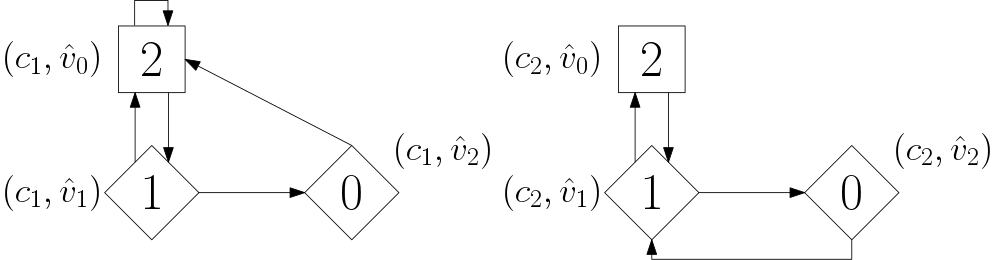
\includegraphics[scale=0.4]{Examples/UPG/UPG}
		\caption{Unified PG, created from unifying the two projections}
	\end{subfigure}
	\caption{A VPG with its corresponding unified PG}
	\label{fig:VPG2UPG}
\end{figure}

If we solve the PG that is the unification of a VPG we have solved the VPG, as shown in the next theorem.
\begin{theorem}
	\label{theA_solve_UVPG_is_solve_VPG}
	Given 
	\begin{itemize}
		\item VPG $\hat{G} =  (\hat{V},\hat{V}_0,\hat{V}_1, \hat{E},\hat{\Omega}, \mathfrak{C},\theta)$,
		\item some configuration $c \in \mathfrak{C}$,
		\item winning sets $\hat{W}^c_0$ and $\hat{W}^c_1$ for game $\hat{G}$ and
		\item winning sets $W_0$ and $W_1$ for game $\hat{G}_{\downarrow}$
	\end{itemize}
	it holds that
	\[(c,\hat{v}) \in W_\alpha \iff \hat{v} \in \hat{W}^c_\alpha  \text{, for }\alpha \in \{0,1\}  \]
	\begin{proof}
		The bi-implication is equal to  the following to implications.
		\[ (c,\hat{v}) \in W_\alpha \implies \hat{v} \in \hat{W}^c_\alpha  \text{, for }\alpha \in \{0,1\} \]
		and
		\[ (c,\hat{v}) \notin W_\alpha\implies \hat{v} \notin \hat{W}^c_\alpha \text{, for }\alpha \in \{0,1\}  \]
		
		Since the winning sets partition the game we have $\hat{v} \notin \hat{W}^c_\alpha \implies \hat{v} \in \hat{W}^c_{\overline{\alpha}}$ (similar for set $W$). Therefore it is sufficient to prove only the first implication.
		
		Let $(c,\hat{v}) \in W_\alpha$, player $\alpha$ has a strategy to win game $\hat{G}_{\downarrow}$ from vertex $(c,\hat{v})$. Since $\hat{G}_{\downarrow}$ is the union of all the projections of $\hat{G}$ we can apply the same strategy to game $\hat{G}_{|c}$ to win vertex $\hat{v}$ as player $\alpha$. Because we can win $\hat{v}$ in the projection of $\hat{G}$ to $c$ we have $\hat{v} \in \hat{W}^c_\alpha$.
	\end{proof}
\end{theorem}

\subsubsection{Projections and totality}
A unified PG can be projected back to one of the games from which it is the union.
\begin{definition}
	The projection of unified PG $G = (V,V_0, V_1,E,{\Omega})$ to configuration $c$, denoted as $G_{|c}$, is the parity game $(V',{V}_0,{V}_1,E',{\Omega})$ such that $V' = \{ {v}\ |\ (c,{v}) \in V \}$ and $E' = \{ ({v},{w})\ |\ ((c,{v}),(c,{w})) \in E \} $.
\end{definition}

One of the properties of a PG is its totality; a game is total if every vertex has at least 1 outgoing vertex. VPGs are also total, meaning that every vertex has, for every configuration $c \in \mathfrak{C}$, at least 1 outgoing vertex admitting $c$. Because VPGs are total their unifications are also total. Since edges in a unified PG don't cross configurations we can conclude that a unified PG is total iff every projection is total.

\subsection{Solving unified PGs}
We can solve a unified PG using Zielonka's recursive algorithm, since it is a total parity game. The algorithm revolves around the attractor operation. Consider the example presented in figure \ref{fig:VPG2UPG}. Vertices with the highest priority are 
\[ \{(c_1,v_0),(c_2,v_0)\}\]
attracting these for player $0$ gives the set 
\begin{align*}
\{(c_1,v_0),&(c_2,v_0),\\
(c_1,v_1),&(c_2,v_1),\\
 &(c_2,v_2)\}
\end{align*}
The algorithm tries to attract all vertices starting from $v_0$ with any configuration, in this case $v_1$ can be attracted for all configurations, $v_2$ can only be attracted for $c_2$. When edge guards are permissive, ie. they admit many configurations, then there is a good change that vertices can be attracted for multiple configurations at the same time during the algorithm. This is the idea for the collective recursive VPG algorithm we present next, we will modify the recursive algorithm to solve unified parity games such that it tries to attract multiple configurations simultaneously.

\subsection{Representing unified parity games}
In order to create an algorithm based around attracting multiple configurations we need to take a look at how unified parity games can be represented.


Unified PGs have a specific structure because they are the union of PGs that have the same vertices with the same owner and priority. Because they have the same priority we don't actually need to create a new function that is the unification of all the projections, we can simply use the original priority assignment function because the following relation holds:
\[ \Omega(c,\hat{v}) = \hat{\Omega}(\hat{v}) \]
Similarly we can use the original partition sets $\hat{V}_0$ and $\hat{V}_1$ instead of having the new partition $V_0$ and $V_1$ because the following relations holds:
\[ (c,\hat{v}) \in V_0 \iff \hat{v}\in \hat{V}_0 \]
\[ (c,\hat{v}) \in V_1 \iff \hat{v}\in \hat{V}_1 \]
So instead of considering unified PG $(V,V_0,V_1,E,\Omega)$ we will consider $(V,\hat{V}_0,\hat{V}_1,E,\hat{\Omega})$. 

Next we consider how we represent vertices and edges in a unified PG. A set $X \subseteq (\mathfrak{C} \times \hat{V})$ can be represented as a complete function $f : \hat{V} \rightarrow 2^\mathfrak{C}$. The set $X$ and function $f$ are equivalent, denoted by the operator $=_\lambda$, iff the following relation holds:
\[ (c,\hat{v}) \in X \iff c \in f(\hat{v}) \]
We can also represent edges as a complete function $f : \hat{E} \rightarrow 2^\mathfrak{C}$. The set $E$ and function $f$ are equivalent, denoted by the operator $=_\lambda$, iff the following relation holds:
\[ ((c,\hat{v}),(c,\hat{v}')) \in E \iff c \in f(\hat{v},\hat{v}') \]
We write $\lambda^\emptyset$ to denote the function that maps every element to $\emptyset$, clearly $\lambda^\emptyset =_\lambda \emptyset$. We call using a set of pairs to represent vertices and edges a \textit{set-wise} representation and using functions a \textit{function-wise} representation.

\subsection{Algorithms}
Using the recursive algorithm as a basis we can solve a VPG independently, alternatively we can solve it collectively using a set-wise presentation or a function-wise presentation. For the function-wise presentation we are working with functions mapping vertices and edges to sets of configurations. These sets of configurations can either be represented explicitly or symbolically. The following diagram shows the different algorithms:
\begin{center}
	\begin{forest}
		[Recursive algorithm, for tree={parent anchor=south, child anchor=north, align=center, s sep=5mm}
		[Independent]
		[Collective
		[Set-wise]
		[Function-wise
		[Explicit]
		[Symbolic]
		]
		]
		]
	\end{forest}
\end{center}
The independent approach uses the original algorithm, the collective set-wise approach also uses the original algorithm applied on a unified PG. The function-wise representation required modifications to the algorithm, as we try to attract multiple configurations at the same time. As we will see, this modified algorithm relies heavily on set operations over sets of configurations. 

\subsubsection{Symbolically representing sets of configurations}
\label{sec:symrepconfs}
For VPGs originating from an FTS the configuration sets are already boolean functions over the features. The formula's guarding the edges in the VPG will generally have relatively simple boolean functions, therefore they are specifically appropriate to represent as BDDs.

A set operation over two explicit sets can be performed in $O(n)$ where $n$ is the maximum size of the sets, this is better than the time complexity of a set operation using BDDs ($O(n^2)$). However if the BDDs are small then the set size can still be large but the set operations can be performed very quickly. This is a trade-off between worst case running time complexity and actual running time; using a symbolic representation might yield better results if the sets are structured in such a way that the BDDs are small, however its worse case running time complexity will be worse.

We hypothesize that since the collective function-wise symbolic recursive algorithm relies heavily on set operations over sets of configurations this algorithm will perform well.

\subsubsection{A note on symbolically solving games}
The function-wise algorithm has two variants: an explicit and a symbolic variant. In the explicit variant everything is represented explicitly. In the symbolic variant the sets of configurations are represented symbolically, however the graph is still represented explicitly so the algorithm is partially symbolic and partially explicit. Alternatively an algorithm could completely work symbolically by representing both the graph and the sets of configurations symbolically.

Solving parity games symbolically has been studied in \cite{BDDSolvingPG}. The obstacle is that representing graphs with a large number of nodes makes the corresponding BDDs very complex and performance decreases rapidly. As to not repeat work done in \cite{BDDSolvingPG} we only consider algorithms where we represent the graph explicitly. 

\subsection{Recursive algorithm using a function-wise representation}
We can modify the recursive algorithm to work with the function-wise representation of vertices and edges. The algorithm behaves the same, only operations are modified to work with the different representation.  Pseudo code for the modified algorithm is presented in algorithm \ref{alg_zlnk_UVPG}. Note that for this pseudo code no distinction is made whether the sets of configurations are represented explicitly or symbolically.
\begin{algorithm}
	\caption{$\textsc{RecursiveUPG}(\textit{PG } G = (\\
		V : \hat{V} \rightarrow 2^\mathfrak{C},\\
		\hat{V}_0 \subseteq \hat{V},\\
		\hat{V}_1 \subseteq \hat{V},\\
		E : \hat{E} \rightarrow 2^\mathfrak{C},\\
		\hat{\Omega} : \hat{V}\rightarrow \mathbb{N}))$}\label{alg_zlnk_UVPG}
	\begin{algorithmic}[1]
		\State $m \gets \min\{ \hat{\Omega}(\hat{v})\ |\ V(\hat{v}) \neq \emptyset \}$
		\State $h \gets \max\{ \hat{\Omega}(\hat{v})\ |\ V(\hat{v}) \neq \emptyset \}$
		\If{$h = m$ or $V = \lambda^\emptyset$}
		\If{$h$ is even or $V = \lambda^\emptyset$}
		\State \Return $(V,\lambda^\emptyset)$
		\Else
		\State \Return $(\lambda^\emptyset, V)$
		\EndIf
		\EndIf
		\State $\alpha \gets 0$ if $h$ is even and $1$ otherwise
		\State $U \gets \lambda^\emptyset$, $U(\hat{v}) \gets V(\hat{v})$ for all $\hat{v}$ with $\hat{\Omega}(\hat{v}) = h$
		\State $A \gets \alpha\textit{-FAttr}(G, U)$
		\State $(W_0', W_1') \gets \textsc{RecursiveUPG}(G \backslash A)$
		\If{$W_{\overline{\alpha}}' =\lambda^\emptyset$}
		\State $W_\alpha \gets A \cup W_\alpha'$
		\State $W_{\overline{\alpha}} \gets \lambda^\emptyset$
		\Else
		\State $B \gets \overline{\alpha}\textit{-FAttr}(G,W_{\overline{\alpha}}')$
		\State $(W_0'', W_1'') \gets \textsc{RecursiveUPG}(G \backslash B)$
		\State $W_\alpha \gets W_\alpha''$
		\State $W_{\overline{\alpha}} \gets W_{\overline{\alpha}}'' \cup B$
		\EndIf
		\State \Return $(W_0, W_1)$
	\end{algorithmic}
\end{algorithm}

We introduce a modified attractor definition to work with the function-wise representation.
\begin{definition}
		\label{def_Uattr}Given unified PG $G = (V, \hat{V}_0,\hat{V}_1,E,\hat{\Omega})$ and a non-empty set $U \subseteq V$, both represented function-wise, we define $\alpha\textit{-FAttr}(G,U)$ such that
	\[U_0 = U \]
	For $i \geq 0$:
	\[
	U_{i+1}(\hat{v}) = U_i(\hat{v}) \cup \begin{cases}
V(\hat{v}) \cap \bigcup_{\hat{v}'} (E(\hat{v},\hat{v}') \cap U_i(\hat{v}')) & \text{if } \hat{v} \in \hat{V_{\alpha}}\\
V(\hat{v}) \cap \bigcap_{\hat{v'}}((\mathfrak{C} \backslash E(\hat{v},\hat{v}')) \cup U_i(\hat{v}') & \text{if }\hat{v} \in  \hat{V_{\overline{\alpha}}} \\
	\end{cases}
	\]
	Finally:
	\[\alpha\textit{-FAttr}(G,U) = \bigcup_{i \geq 0} U_i \]
\end{definition}
We now prove that the function-wise attractor definition gives a result equal to the original definition.
\begin{lemma}
	\label{lem_attr_equal}
	Given unified PG $G = (\mathcal{V},\hat{V}_0,\hat{V}_1, \mathcal{E}, \hat{\Omega})$ and set $\mathcal{U} \subseteq \mathcal{V}$ the function-wise attractor $\alpha\textit{-FAttr}(G,\mathcal{U})$ is equivalent to the set-wise attractor $\alpha\textit{-Attr}(G,\mathcal{U})$ for any $\alpha \in \{0,1\}$.
	\begin{proof}
		Let $V,E,U$ be the set-wise representation and $V^\lambda,E^\lambda,U^\lambda$ be the function-wise representation of $\mathcal{V},\mathcal{E},\mathcal{U}$ respectively.
		
		The following properties hold by definition:
		\[ (c,\hat{v}) \in V \iff c \in V^\lambda(\hat{v})\]
		\[ (c,\hat{v}) \in U \iff c \in U^\lambda(\hat{v})\]
		\[ ((c,\hat{v}),(c,\hat{v}')) \in E \iff c \in E^\lambda(\hat{v},\hat{v}') \]
		
		Since the attractors are inductively defined and $U_0 =_\lambda U^\lambda_0$ (because $U =_\lambda U^\lambda$) we have to prove that for some $i \geq 0$, with $U_i =_\lambda U^\lambda_i$,  we have $U_{i+1} =_\lambda U^\lambda_{i+1}$, which holds iff:
		\[ (c,\hat{v}) \in U_{i+1} \iff c \in U^\lambda_{i+1}(\hat{v}) \]
		Let $(c,\hat{v}) \in V$ (and therefore $c \in V^\lambda(\hat{v})$), we consider 4 cases.
		\begin{itemize}
			\item Case: $\hat{v} \in \hat{V}_{\alpha}$ and $(c,\hat{v}) \in U_{i+1}$:\\
			To prove: $c \in U^\lambda_{i+1}(\hat{v})$.
			
			If $(c,\hat{v}) \in U_i$ then $c \in U^\lambda_i(\hat{v})$ and therefore $c \in U^\lambda_{i+1}(\hat{v})$. If $(c,\hat{v}) \notin U_i$ then we have $c \notin U^\lambda_i(\hat{v})$.
			
			
			Because $\hat{v} \in \hat{V}_{\alpha}$ and $c \in V^\lambda(\hat{v})$ we get
			\[ U^\lambda_{i+1} =\bigcup_{\hat{v}'} (E^\lambda(\hat{v},\hat{v}') \cap U^\lambda_i(\hat{v}')) \]
			
			There exists an $(c',\hat{v}') \in V$ such that $(c',\hat{v}') \in U_i$ and $((c,\hat{v}),(c',\hat{v}')) \in E$. Because edges don't cross configurations we can conclude that $c' = c$. Due to equivalence we have $c \in U^\lambda_i(\hat{v}')$ and $c \in E^\lambda(\hat{v},\hat{v}')$. If we fill this in in the above formula we can conclude that $c \in U^\lambda_{i+1}(\hat{v})$.
			\item Case: $\hat{v} \in \hat{V}_{\alpha}$ and $(c,\hat{v}) \notin U_{i+1}$:\\
			To prove: $c \notin U^\lambda_{i+1}(\hat{v})$.
			
			
			First we observe that since $(c, \hat{v}) \notin U_{i+1}$ we get $(c, \hat{v}) \notin U_{i}$ and therefore $c \notin U^\lambda_i(\hat{v})$.
			
			Because $\hat{v} \in \hat{V}_{\alpha}$ and $c \in V^\lambda(\hat{v})$ we get
\[ U^\lambda_{i+1} =\bigcup_{\hat{v}'} (E^\lambda(\hat{v},\hat{v}') \cap U^\lambda_i(\hat{v}')) \]
			
			Assume $c \in U^\lambda_{i+1}(\hat{v})$. There must exist a $\hat{v}'$ such that $c \in E^\lambda(\hat{v},\hat{v}')$ and $c \in U^\lambda_i(\hat{v}')$. Due to equivalence we have a vertex $((c,\hat{v}),(c,\hat{v}')) \in E$ and $(c,\hat{v}') \in U_i$. In which case $(c,\hat{v})$ would be attracted and would be in $U_{i+1}$ which is a contradiction.
			\item Case: $\hat{v} \in \hat{V}_{\overline{\alpha}}$ and $(c,\hat{v}) \in U_{i+1}$:\\
			To prove: $c \in U^\lambda_{i+1}(\hat{v})$.
			
			If $(c,\hat{v}) \in U_i$ then $c \in U^\lambda_i(\hat{v})$ and therefore $c \in U^\lambda_{i+1}(\hat{v})$. If $(c,\hat{v}) \notin U_i$ then we have $c \notin U^\lambda_i(\hat{v})$.
			
			Because $\hat{v} \in \hat{V}_{\overline{\alpha}}$ we get
			\[ U^\lambda_{i+1} =V^\lambda(\hat{v}) \cap \bigcap_{\hat{v'}}((\mathfrak{C} \backslash E^\lambda(\hat{v},\hat{v}')) \cup U^\lambda_i(\hat{v}') \]
			
			Assume $c \notin U^\lambda_{i+1}(\hat{v})$. Because $c \in V^\lambda(\hat{v})$ there must exist an $\hat{v}$ such that
			\[ c \notin ((\mathfrak{C} \backslash E^\lambda(\hat{v},\hat{v}')) \text{ and } c \notin U^\lambda_i(\hat{v}') \]
			which is equal to
			\[ c \in E^\lambda(\hat{v},\hat{v}') \text{ and } c \notin U^\lambda_i(\hat{v}') \]
			By equivalence we have $((c,\hat{v}),(c,\hat{v}')) \in E$ and $(c,\hat{v}') \notin U_i$. Which means that $(c,\hat{v})$ will not be attracted and $(c,\hat{v}) \notin U_{i+1}$ which is a contradiction.
			\item Case: $\hat{v} \in \hat{V}_{\overline{\alpha}}$ and $(c,\hat{v}) \notin U_{i+1}$:\\
			To prove: $c \notin U^\lambda_{i+1}(\hat{v})$.
			
			First we observe that since $(c, \hat{v}) \notin U_{i+1}$ we get $(c, \hat{v}) \notin U_{i}$ and therefore $c \notin U^\lambda_i(\hat{v})$.
			
			Because $\hat{v} \in \hat{V}_{\overline{\alpha}}$ we get
			\[ U^\lambda_{i+1} =V^\lambda(\hat{v}) \cap \bigcap_{\hat{v'}}((\mathfrak{C} \backslash E^\lambda(\hat{v},\hat{v}')) \cup U^\lambda_i(\hat{v}') \]
			
			Since $(c,\hat{v})$ is not attracted there must exist a $(c,\hat{v}') \in V$ such that 
			\[ ((c,\hat{v}),(c,\hat{v}')) \in E  \text{ and } (c,\hat{v}') \notin U_i \]
			By equivalence we have 
			\[ c \in E^\lambda(\hat{v},\hat{v}')  \text{ and } c \notin U^\lambda_i(\hat{v}') \]
			Which is equal to
			\[ c \notin (\mathfrak{C} \backslash E^\lambda(\hat{v},\hat{v}'))  \text{ and } c \notin U^\lambda_i(\hat{v}') \]
			From which we conclude
			\[ c \notin ((\mathfrak{C} \backslash E^\lambda(\hat{v},\hat{v}')) \cup U^\lambda_i(\hat{v}'))) \]
			Therefore we have $c \notin U^\lambda_{i+1}(\hat{v})$.
		\end{itemize}
	\end{proof}
\end{lemma}

We also introduce a modified subgame definition to work with the function-wise representation.
\begin{definition}
	\label{def_Usubgame}
	For unified PG $G = (V,\hat{V}_0,\hat{V}_1,E,\hat{\Omega})$, represented function-wise, and set $X \subseteq V$ we define the subgame $G \backslash X = (V',\hat{V}_0,\hat{V}_1,E',\hat{\Omega})$ such that:
	\begin{itemize}
		\item $V'(\hat{v}) = V(\hat{v}) \backslash X(\hat{v})$
		\item $E'(\hat{v},\hat{v}') = E(\hat{v},\hat{v}') \cap V'(\hat{v}) \cap V'(\hat{v}')$
	\end{itemize}
\end{definition}
We prove that this new subgame definition gives a result equal to the original subgame definition. Note that when using the original subgame definition for unified PGs we can omit the modification to the partition because, as we have seen, we can use the partitioning from the VPG in the representation of unified PGs.
\begin{lemma}
	\label{lem_subgame_eq}
	Given unified PG $G = (\mathcal{V},\hat{V}_0,\hat{V}_1, \mathcal{E}, \hat{\Omega})$ and set $\mathcal{U} \subseteq \mathcal{V}$ the subgame $G \backslash \mathcal{U} = (\mathcal{V}',\hat{V}_0,\hat{V}_1,\mathcal{E}',\hat{\Omega})$ represented set-wise is equal to the subgame represented function-wise.
	\begin{proof}
		Let $V,V',E,E',U$ be the set-wise and $V^\lambda,{V^\lambda}', E^\lambda, {E^\lambda}', U^\lambda$ the function-wise representations of $\mathcal{V},\mathcal{V}', \mathcal{E}, \mathcal{E}', \mathcal{U}$ respectively. We know $V =_\lambda V^\lambda$, $E =_\lambda E^\lambda$ and $U =_\lambda U^\lambda$. To prove: $V' =_\lambda {V^\lambda}'$ and $E' =_\lambda {E^\lambda}'$.
		
		Let $(c,\hat{v}) \in V$.
		
		If $(c,\hat{v}) \in U$ then $c \in U^\lambda(\hat{v})$, also $(c,\hat{v}) \notin V'$ (by definition \ref{def_org_subgame}) and $c \notin {V^\lambda}'(\hat{v})$ (by definition \ref{def_Usubgame}).
		
		If $(c,\hat{v}) \notin U$ then $c \notin U^\lambda(\hat{v})$, also $(c,\hat{v}) \in V'$ (by definition \ref{def_org_subgame}) and $c \in {V^\lambda}'(\hat{v})$ (by definition \ref{def_Usubgame}).
		
		Let $((c,\hat{v}),(c,\hat{w})) \in E$.
		
		If $(c,\hat{v}) \in U$ then $(c,\hat{v}) \notin V'$ and $c \notin {V^\lambda}'(\hat{v})$ (as shown above). We get $((c,\hat{v}),(c,\hat{w})) \notin V' \times V'$ so $((c,\hat{v}),(c,\hat{w})) \notin E'$ (by definition \ref{def_org_subgame}). Also $c \notin {E^\lambda}'(\hat{v},\hat{w})$ (by definition \ref{def_Usubgame}).
		
		If $(c,\hat{w}) \in U$ then we apply the same logic.
		
		If neither is in $U$ then both are in $V'$ and in $V' \times V'$ and therefore the $((c,\hat{v}),(c,\hat{w})) \in E'$. Also we get $c \in {V^\lambda}'(\hat{v})$ and $c \in {V^\lambda}'(\hat{w})$ so we get $c \in {E^\lambda}'(\hat{v},\hat{w})$ (by definition \ref{def_Usubgame}).
	\end{proof}
\end{lemma}

Next we prove the correctness of the algorithm by showing that the winning sets of the function-wise algorithm are equal to the winning sets of the set-wise algorithm.
\begin{theorem}
	Given unified PG $\mathcal{G} = (\mathcal{V},\hat{V}_0,\hat{V}_1, \mathcal{E}, \hat{\Omega})$ the winning sets resulting from \textsc{RecursiveUPG($\mathcal{G}$)} ran over the function-wise representation of $\mathcal{G}$ is equal to the winning sets resulting from \textsc{RecursivePG($\mathcal{G}$)} ran over the set-wise representation of $\mathcal{G}$.
	\begin{proof}
		Let $G = (V,\hat{V}_0,\hat{V}_1,E,\hat{\Omega})$ be the set-wise representation of $\mathcal{G}$ and $G^\lambda = (V^\lambda, \hat{V}_0, \hat{V}_1, E^\lambda, \hat{\Omega})$ be the function-wise representation of $\mathcal{G}$.
		
		Proof by induction on $\mathcal{G}$.
		
		\textbf{Base} When there are no vertices or only one priority \textsc{RecursiveUPG($G^\lambda$)} returns $\lambda^\emptyset$ and \textsc{RecursivePG($G$)} returns $\emptyset$, these two results are equal therefore the theorem holds in this case.
		
		\textbf{Step}
		Player $\alpha$ gets the same value in both algorithms since the highest priority is equal for both algorithms.
		
		Let $U = \{(c,\hat{v}) \in V\ |\ \hat{\Omega}(\hat{v}) = h \}$ (as calculated by \textsc{RecursivePG}) and $U^\lambda(\hat{v}) = V^\lambda(\hat{v})$ for all $\hat{v}$ with $\hat{\Omega}(\hat{v}) = h$ (as calculated by \textsc{RecursiveUPG}). We will show that $U =_\lambda U^\lambda$.
		
		Let $(c,\hat{v}) \in U$ then $\hat{\Omega}(\hat{v}) = h$, therefore $U^\lambda(\hat{v}) = V^\lambda(\hat{v})$. Since $U \subseteq V$ we have $(c,\hat{v}) \in V$ and because the equality between $V$ and $V^\lambda$ we get $c \in V^\lambda(\hat{v})$ and $c \in U^\lambda(\hat{V})$.
		
		Let $c \in U^\lambda(\hat{v})$, since $U^\lambda(\hat{v})$ is not empty we have $\hat{\Omega}(\hat{v}) = h$, furthermore $c \in V^\lambda(\hat{v})$ and therefore $(c,\hat{v}) \in V$. We can conclude that $(c, \hat{v}) \in U$ and $U =_\lambda U^\lambda$.
		
		For the rest of the algorithm it is sufficient to see that attractor sets are equal if the game and input set are equal (as shown in lemma \ref{lem_attr_equal}) and that the created subgames are equal (as shown in lemma \ref{lem_subgame_eq}). Since the subgames are equal we can apply the theorem on it by induction and conclude that the winning sets are also equal.
	\end{proof}
\end{theorem}

Theorem \ref{theA_solve_UVPG_is_solve_VPG} shows that solving a unified PG solves the VPG, furthermore the algorithm \textsc{RecursiveUPG} correctly solves a unified PG therefore we can conclude that for VPG $\hat{G}$ vertex $\hat{v}$ is won by player $\alpha$ for configuration $c$ iff $c \in W_\alpha(\hat{v})$ with $(W_0,W_1) = \textsc{RecursiveUPG}(G_{\downarrow})$.

\subsubsection{Function-wise attractor set}
Next we present an algorithm to calculate the function-wise attractor, the pseudo code is presented in algorithm \ref{alg_fattr_alg}. The algorithm considers vertices that are in the attracted set for some configuration, for every such vertex the algorithm tries to attract vertices that are connected by an incoming edge. If a vertex is attracted for some configuration then the incoming edges of that vertex will also be considered. We prove the correctness of the algorithm in the following lemma and theorem.
\begin{algorithm}
	\caption{$\textsc{$\alpha$-FAttractor}(G, A : \hat{V} \rightarrow 2^\mathfrak{C})$}\label{alg_fattr_alg}
	\begin{algorithmic}[1]
		\State Queue $Q \gets \{\hat{v} \in \hat{V} \ |\ A(\hat{v}) \neq \emptyset  \}$
		\While{$Q$ is not empty}
		\State $\hat{v}' \gets Q.pop()$
		\For{$E(\hat{v},\hat{v}') \neq \emptyset$}
			\If{$\hat{v} \in \hat{V}_\alpha$}
				\State $a \gets V(\hat{v}) \cap E(\hat{v},\hat{v}') \cap A(\hat{v}')$
			\Else
				\State $a \gets V(\hat{v})$
				\For{$E(\hat{v},\hat{v}'') \neq \emptyset$}
					\State $a \gets a \cap (\mathfrak{C}\backslash E(\hat{v},\hat{v}'') \cup A(\hat{v}''))$
				\EndFor
			\EndIf
			\If{$a \backslash A(\hat{v}) \neq \emptyset$}
				\State $A(\hat{v}) \gets A(\hat{v}) \cup a$
				\State $Q.push(\hat{v})$
			\EndIf
		\EndFor
		\EndWhile
		\State \Return $A$
	\end{algorithmic}
\end{algorithm}
\begin{lemma}
\label{lem_attr_requires_E}
Vertex $\hat{v}$ and configuration $c$, with $c \in V(\hat{v})$, can only be attracted if there is a vertex $\hat{v}'$ such that $c \in E(\hat{v}, \hat{v}')$ and $c \in U_i(\hat{v}')$.
	\begin{proof}
		We first observe that if $\hat{v} \in \hat{V}_\alpha$ then this property follows immediately from definition the function-wise attractor definition (\ref{def_Uattr}). If $\hat{v} \in \hat{V}_{\overline{\alpha}}$ we note that unified PGs are total and therefore all of their projections are also total. So vertex $\hat{v}$ has at least one outgoing edge for $c$, we have $\hat{w}$ such that $c \in E(\hat{v},\hat{w})$. For $\hat{v}$ with $c$ to be attracted we must have $c \in U_i(\hat{w})$.
	\end{proof}
\end{lemma}
\begin{theorem}
Set $A$ calculated by $\textsc{$\alpha$-FAttractor}(G,U)$ satisfies $A = \alpha\textit{-FAttr}(G,U)$.
	\begin{proof} We will prove two loop invariants over the while loop of the algorithm.
		
		\textbf{IV1}: For every $\hat{w} \in \hat{V}$ and $c \in \mathfrak{C}$ with $c \in A(\hat{w})$ we have $c \in \alpha\textit{-FAttr}(G,U)(\hat{w})$.
		
		\textbf{IV2}: For every $\hat{w} \in \hat{V}$ and $c \in \mathfrak{C}$ that can be attracted to $A$ either $c \in A(\hat{w})$ or there exists a $\hat{w}' \in Q$ such that $c \in E(\hat{w},\hat{w}')$.
		
		\textbf{Base}: Before the loop starts we have $A = U$, therefore IV1 holds. Furthermore all the vertices that are in $A$ for some $c$ are also in $Q$ so IV2 holds.
		
		\textbf{Step}: Consider the beginning of an iteration and assume IV1 and IV2 hold. To prove: IV1 and IV2 hold at the end of the iteration.
		
		Set $A$ only contains vertices with configurations that are in $\alpha\textit{-FAttr}(G,U)$. The set is only updated through lines 5-12 and 14 of the algorithm which reflects the exact definition of the attractor set therefore IV1 holds at the end of the iteration.
		
		Consider $\hat{w} \in \hat{V}$ and $c \in \mathfrak{C}$, we distinguish three cases to prove IV2:
		\begin{itemize}
			\item $\hat{w}$ with $c$ can be attracted by the beginning of the iteration but not by the end.
			
			This case can't happen because $A(\hat{w})$ only increases during the algorithm and the values for $E$ and $V$ are not changed throughout the algorithm.
			\item $\hat{w}$ with $c$ can't be attracted by the beginning of the iteration but can by the end.
			
			For $\hat{w}$ with $c$ to be able to be attracted at the end of the iteration there must be some $\hat{w}'$ with $c$ such that during the iteration $c$ was added to $A(\hat{w}')$ (lemma \ref{lem_attr_requires_E}). Every $\hat{w}'$ for which $A(\hat{w}')$ is updated is added to the queue (lines 13-16). Therefore we have $\hat{w}' \in Q$ with $c \in E(\hat{w},\hat{w}')$ and IV1 holds.
			\item $\hat{w}$ with $c$ can be attracted by the beginning of the iteration and also by the end.
			
			Since IV2 holds at the beginning of the iteration we have either $c \in A(\hat{w})$ or we have some $\hat{w}' \in Q$ such that $c \in E(\hat{w},\hat{w}')$. In the former case IV2 holds trivially by the end of the iteration since $A(\hat{w})$ can only increase. For the latter case we distinguish two scenario's. 
			
			First we consider the scenario where vertex $\hat{v}'$ that is considered during the iteration (line 3 of the algorithm) is $\hat{w}'$. There is a vertex $c \in E(\hat{w},\hat{w}')$ by IV2. Therefore we can conclude that $\hat{w}$ is considered in the for loop starting at line $4$ and will be attracted in lines 5-12 and added to $A(\hat{w})$ in line 14. Therefore IV2 holds by the end of the iteration.
			
			Next we consider the scenario where $\hat{v}' \neq \hat{w}'$. In this case by the end of the iteration $\hat{w}'$ will still be in $Q$ and IV2 holds.
		\end{itemize}
	
	Vertices are only added to the queue when something is added to $A$ (if statement on line 13). This can only finitely often happen because $A(\hat{v})$ can never be larger than $V(\hat{v})$ so we can conclude that the while loop terminates after a finite number of iterations.
	
		When the while loop terminates IV1 and IV2 hold so for every $\hat{w} \in \hat{V}$ and $c \in \mathfrak{C}$ that can be attracted to $A$ we have $c \in A(\hat{w})$. Since we start with $A = U$ we can conclude the soundness of the algorithm. IV1 shows the completeness.
	\end{proof}
\end{theorem}


\subsection{Running time}
We will consider the running time for solving VPG $G = (V,V_0,V_1,E,\Omega,\mathfrak{C},\theta)$ independently and collectively using the different types of representations. Let $n$ denote the number of vertices, $e$ the number of edges, $c$ the number of configurations and $d$ the number of distinct priorities.

The original algorithm runs in $O(e * n^d)$, if we run $c$ parity games independently we get $O(c * e * n ^d)$. We can also apply the original algorithm to a unified PG (represented set-wise) for a collective approach, in this case we get a parity game with $c*n$ vertices and $c*e$ edges. which gives a running time $O(c*e*(c*n)^d)$. However this running time can be improved by using the property that a unified PG consists of $c$ disconnected graphs as we show next.

We have introduced three types of collective algorithms: set-wise, function-wise with explicit configuration sets and function-wise with symbolic configuration sets. In all three algorithms the running time of the attractor set is dominant, so we need three things: analyse the running time of the base cases, analyse the running time of the attractor set and analyse the recursion.

\textit{Base cases.} In the base cases the algorithm needs to do two things: find the highest and lowest priority and check if there are no more vertices in the game. For the set-wise variant we find the highest and lowest priorities by iterating all vertices, which takes $O(c*n)$. Checking if there are no more vertices is done in $O(1)$. For the function wise algorithms we can find the highest and lowest priority in $O(n)$ and checking if there are no vertices is also done in $O(n)$ since we have to check $V(\hat{v}) = \emptyset$ for every $\hat{v}$. Note that in a symbolic representation using BDDs we can check if a set is empty in $O(1)$ because the decision diagram contains a single node.

\textit{Attractor sets.} For the set-wise collective approach we can use the attractor calculation from the original algorithm which has a time complexity of $O(e)$, so for a unified PG having $c*e$ edges we have $O(c*e)$.

The function-wise variants use a different attractor algorithm. First we consider the variant where sets of configurations are represented explicitly.

Consider algorithm \ref{alg_fattr_alg}. A vertex will be added to the queue when this vertex is attracted for some configuration, this can only happen $c*n$ times, once for every vertex configuration combination. 

The first for loop considers all the incoming edges of a vertex. When we consider all vertices the for loop will have considered all edges, since we consider every vertex at most $c$ times the for loop will run at most $c*e$ times in total.

The second for loop considers all outgoing edges of a vertex. The vertices that are considered are the vertices that have an edge going to the vertex being considered by the while loop. Since the while loop considers $c*n$ vertices the second for loop runs in total at most $c * n * e$ times. The loop itself performs set operations on the set of configurations which can be done in $O(c)$. This gives a total time complexity for the attractor set of $O(n*c^2*e)$.

For the symbolic representation set operations can be done in $O(c^2)$ so we get a time complexity of $O(n*c^3*e)$.

This gives the following time complexities\\
\begin{center}
	\begin{tabular}{|c|c|c|}
		\hline 
		& Base & Attractor set \\ 
		\hline 
		Set-wise & $O(c*n)$ & $O(c*e)$  \\ 
		\hline 
		Function-wise explicit & $O(n)$ &  $O(n*c^2*e)$ \\ 
		\hline 
		Function-wise symbolic & $O(n)$ &  $O(n* c^3*e)$ \\ 
		\hline 
	\end{tabular} 
\end{center}

\textit{Recursion}. The three algorithms behave the same way with regards to their recursion, so we analyse the running time of the set-wise variant and can derive the time complexity of the others using the result.

The algorithm has two recursions, the first recursion lowers the number of distinct priorities by 1. The second recursion removes at least one edge, however the game is comprised of disjoint projections. We can use this fact use in the analyses. Consider unified PG $G$ and $A$ as specified by the algorithm. Now consider the projection of $G$ to an arbitrary configuration $q$, $G_{|q}$. If $(G\backslash A)_{|q}$ contains a vertex that is won by player $\overline{\alpha}$ then this vertex is removed in the second recursion step. If there is no vertex won by player $\overline{\alpha}$ then the game is won in its entirety and the only vertices won by player $\overline{\alpha}$ are in different projections. We can conclude that for every configuration $q$ the second recursion either removes a vertex or $(G\backslash A)_{|q}$ is entirely won by player $\alpha$. Let $\overline{n}$ denote be the maximum number of vertices that are won by player $\overline{\alpha}$ in game $(G\backslash A)_{|q}$. Since every projection has at most $n$ vertices the value for $\overline{n}$ can be at most $n$. Furthermore since $\overline{n}$ depends on $A$, which depends on the maximum priority, the value $\overline{n}$ gets reset when the top priority is removed in the first recursion. We can now write down the recursion of the algorithm:
\[ T(d,\overline{n}) \leq T(d-1,n) + T(d, \overline{n} - 1) + O(c*e) \]
When $\overline{n} = 0$ we will get $W_{\overline{\alpha}} = \emptyset$ as a result of the first recursion. In such a case there will be only 1 recursion.
\[ T(d,0) \leq T(d-1,n) + O(c*e) \]
Finally we have the base case where there is 1 priority:
\[ T(1, \overline{n}) \leq O(c*n) \]
Expanding the second recursion gives
\begin{align*}
T(d) &\leq (n+1)T(d-1) + (n+1)O(c*e)\\
T(1) &\leq O(c*n)
\end{align*}
We will now prove that $T(d) \leq (n+d)^dO(c*e)$ by induction on $d$.

\textbf{Base} $d=1$: $T(1) \leq O(c*n) \leq O(c*e) \leq (n+1)^1O(c*e)$

\textbf{Step} $d > 1$:
\begin{align*}
T(d) &\leq (n+1)T(d-1) + (n+1)O(c*e)\\
&\leq (n+1)(n+d-1)^{d-1}O(c*e) + (n+1)O(c*e)
\end{align*}
Since $n+1 \leq n+d-1$ we get:
\begin{align*}
T(d) &\leq (n+d-1)(n+d-1)^{d-1}O(c*e) + (n+1)O(c*e)\\
&\leq (n+d-1)^dO(c*e) + (n+1)O(c*e)\\
&\leq ((n+d-1)^d + n + 1)O(c*e)
\end{align*}
Using lemma \ref{lem_md_ineq} we get
\begin{align*}
T(d) &\leq (n+d)^dO(c*e)
\end{align*}
This gives a time complexity of $O(c*e*(n+d)^d) = O(c*e*n^d)$. Note that the base time complexity is subsumed in the recursion by the time complexity of the attractor set. Since the time complexity of the attractor set is higher that the time complexity of the base cases for all three variants of algorithms we can simply fill in the attractor time complexity to get $O(n*c^2*e*n^d)$ for the function-wise explicit algorithm and $O(n*c^3*e*n^d)$ for the function-wise symbolic algorithm.

The different algorithms, including their time complexities, are repeated in the diagram below:\\
\begin{center}
	\begin{forest}
	[Recursive algorithm, for tree={parent anchor=south, child anchor=north, align=center, s sep=5mm}
		[Independent\\$O(c*e*n^d)$ ]
		[Collective
			[Set-wise\\$O(c*e*n^d)$ ]
			[Function-wise
				[Explicit\\$O(n * c^2 * e * n^d)$ ]
				[Symbolic\\$O(n * c^3 * e * n^d)$ ]
			]
		]
	]
	\end{forest}
\end{center}

\subsubsection{Running time in practice}
Earlier we hypothesized that the symbolic function-wise algorithm could have the best performance of the 4 algorithms, however it has the worse case running time complexity. Our hypothesis was based on the notion that VPGs most likely have a lot of commonalities and that sets of configurations in the VPG can be represented efficiently symbolically. Next we argue why the worse case running time complexity might not represent the running time in practice.

We dissect the running time of the function-wise algorithms. The running time complexities of the collective algorithms consist of two parts: the time complexity of the attractor set times $n^d$. The function-wise attractor set time complexity also consists of two parts: the maximum number of vertices in the queue ($c*n$) times the time complexity for set operations ($O(c)$ for the explicit variant, $O(c^2)$ for the symbolic variant).

The number of vertices in the queue during attracting is at most $c*n$, however this number will only be large if we attract a very small number of configurations per time we evaluate an edge. As argued earlier we can most likely attract multiple configurations at the same time. This will decrease the number of vertices in the queue.

The time complexity of set operations is $O(c)$ when using an explicit representation and $O(c^2)$ when using a symbolic one. However, as shown in \cite{BDD_running_time}, a breadth-depth first implementation of BDDs keeps a table of already computed results. This allows us to get already calculated results in sublinear time. In total there are $2^c$ possible sets and therefore $2^{2c}$ possible set combinations and $O(2^c)$ possible set operations that can be computed. However when solving a VPG originating from an FTS there will most likely be a relatively small number of different edge guards, in which case the number of unique sets considered in the algorithm will be small and we can often retrieve a set calculation from the computed table.

We can see that even though the running time of the collective symbolic algorithm is the worse, its practical running time might be good when we are able to attract multiple configurations at the same time and have a small number of different edge guards.